
\section{Linealización}



    Supongamos que $f:\R\to\R$ es diferenciable en $a\in\R,$ es decir, existe la derivada $f'(a).$ Como ya hemos visto,
    esta derivada es la \emph{pendiente} de la \emph{recta tangente,} que es la mejor \emph{aproximación
        lineal} de $f$ en $a.$



    La ecuación de la recta tangente se puede obtener a partir de la siguiente ecuación:
    $$
    \dfrac{y-f(a)}{x-a}=f'(a),
    $$
    que es la ecuación de una recta que pasa por el punto $(a,f(a))$ con pendiente $f'(a).$



    \begin{definicion}
        Sea $f:\R \to \R$ una función diferenciable. Definimos la \emph{linealización} de $f$ alrededor de (o con pivote en)
        $a\in \R$ como
        $$
        L_{f,a}(x)=f(a)+f'(a)(x-a).
        $$
    \end{definicion}



    La linealización $L_{f,a}(x)$ se puede usar para hacer calcular de manera bastante precisa de valor de $f(x)$ para
    $x\approx a.$


{Aproximación de la raíz cuadrada}
    
    \begin{figure}
        \centering
        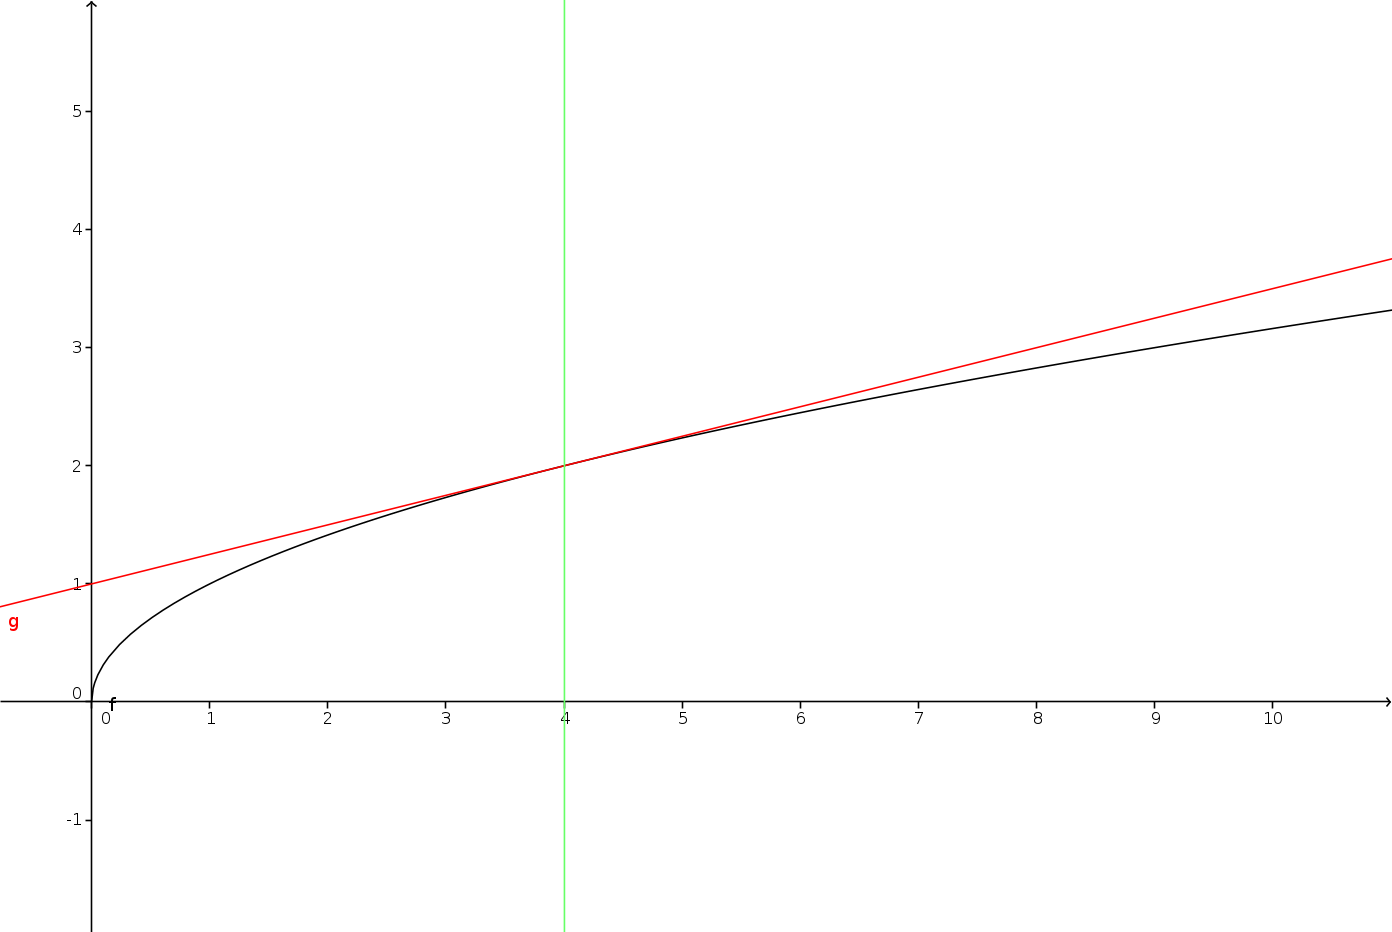
\includegraphics[height=3cm,keepaspectratio=true]{./calculo/sqrt-linear.png}
        % sqrt-linear.png: 1392x932 pixel, 300dpi, 11.79x7.89 cm, bb=0 0 334 224
        \caption{Linealización de $\sqrt{x}$ alrededor $a=4.$}
        \label{fig:sqrt}
    \end{figure}



    Existen varios algoritmos para calcular la raíz de un número real. Sin embargo, podemos calcular raíces de números
    reales de manera muy precisa, usando la linealización.



    Por ejemplo, calculemos $\sqrt{4.1}.$ Primero determinamos la función a linealizar, en este caso, $f(x)=\sqrt{x}.$ La
    derivada de $f$ es
    $$
    f'(x)=\dfrac{1}{2\sqrt{x}}.
    $$



    Después, escogemos como pivote el punto $a=4.$ En este caso $f(4)=2$ y $f'(4)=\frac{1}{4}.$ De donde obtenemos
    
    $$
    L(x)=f(4)+f'(4)(x-4)=2+\frac{1}{4}(x-4).
    $$



    Entonces
    $$
    \sqrt{4.1}\approx L(4.1) =2+.25(4.1-4)=2.025.
    $$



    Si usáramos una calculador, obtendríamos $\sqrt{4.1}=2.02484567313.$



    El error absoluto entre este valor y el que
    obtuvimos de la aproximación es
    $$
    \abs{2.025-2.02484567313}\approx 1.54 \times 10^{-4}.
    $$
    



    
    \begin{problema}
        Use una aproximación lineal para calcular los siguientes valores. Posteriormente, use una calculadora para encontrar
        su valor y determine el error absoluto.
        \begin{enumerate}
            \item $(2.001)^{5}$
            \item $e^{-0.015}$
            \item $(8.06)^{2/3}$
            \item $\frac{1}{1002}$
            \item $\tan(44^{o})$
            \item $\sqrt{99.8}$
        \end{enumerate}
        
    \end{problema}

